\documentclass[11pt,a4paper]{article}
\usepackage[utf8]{inputenc}
\usepackage[T1]{fontenc}
\usepackage{amsmath,amssymb,amsthm}
\usepackage{graphicx}
\usepackage[margin=2.5cm]{geometry}
\usepackage{hyperref}
\usepackage{xcolor}
\usepackage{booktabs}
\usepackage{authblk}
\usepackage{cite}
\hypersetup{colorlinks=true,linkcolor=blue,citecolor=blue,urlcolor=blue}

\title{\textbf{Discrete Drainage Dynamics IV:\\
Light Deflection, Shapiro Delay, and the Photon-Substrate Coupling\\
in the Static Spherical Sector\\[0.4em]
\Large\itshape A phenomenological calibration of the spatial bandwidth coupling}}
\author[1]{Stanislas Dewavrin}
\affil[1]{Independent researcher \\ \texttt{dewavrin.iphone@gmail.com}}
\date{April 2026}

\begin{document}
\maketitle

\begin{abstract}
\noindent
\textbf{Discrete Drainage Dynamics (DDD) is an analogue-substrate
programme.} It does not contest General Relativity: GR is the
empirical anchor any analogue must reproduce in the
appropriate weak-field, static spherical limit. We ask the
exploratory question of whether two canonical weak-field GR
observables --- light deflection and Shapiro delay --- can
emerge from the discrete toy substrate of Papers~II and~III
under a phenomenological photon-substrate coupling.

Paper~II derived a static spherical bandwidth profile
$R(r)/R_0 = \sqrt{1 - \beta/r}$ and identified its time
component with a Schwarzschild-like clock-rate factor. Paper~III
introduced the spinor sector and recovered the Lorentz kinematic
factor at moving wavepackets. Here we ask the next question: does
DDD reproduce the gravitational propagation observables --- light
deflection $4GM/c^2 b$ and the Shapiro time delay --- in the same
static spherical sector? We do not derive the photon sector from
the substrate dynamics; that is deferred to Paper~VI. We adopt a
phenomenological coupling, $c_{\rm eff}(r) = c\,(R/R_0)^\eta$,
and test two ansatze: $\eta = 1$ (temporal only) and
$\eta = 2$ (temporal $+$ spatial). Numerical ray-tracing through
the Paper~II profile gives, for $\eta = 2$, asymptotic
convergence to the GR predictions $\Delta\theta = 4GM/c^2 b$
(deflection) and $c\,\Delta T = (4GM/c^2)\ln(\cdots)$ (Shapiro);
in our numerical setup the Shapiro delay reaches sub-percent
agreement near $b/\beta \sim 50$, the deflection near
$b/\beta \sim 500$, with finite-impact-parameter corrections
behaving as $\sim 2.4\,\beta/b$ in both observables. The
$\eta = 1$ ansatz gives exactly half the GR values, ruled out
by data at the factor-of-two level. The
choice $\eta = 2$ is the substrate analogue of the
spatial-component contribution of the Schwarzschild metric;
$\eta = 1$ would be the prediction if the spatial part of the
substrate were rigid. Within this two-member ansatz family the
data falsify $\eta = 1$ and select $\eta = 2$. Following the
hypothesis terminology established in Paper~III, we adopt
$\eta = 2$ as a structural \emph{hypothesis} of the
photon-substrate coupling, not as a derived consequence: the
substrate principles fix the temporal component
$g_{tt} \propto (R/R_0)^2$, but the spatial component remains
to be derived. The microscopic mechanism that selects
$\eta = 2$ over other spatial choices is the principal open
problem of the gravitational sector.
\end{abstract}


\noindent\fbox{\parbox{0.96\textwidth}{\small
\textbf{What this paper makes mechanically legible.}
GR predicts the famous factor of two between Newtonian and
relativistic light deflection ($4GM/c^2 b$ vs $2GM/c^2 b$) as a
consequence of the spatial component of the Schwarzschild
metric; the metric prescription is precise but supplies no
mechanism for \emph{why} the spatial measure should be throttled
by the same factor as the temporal measure. \emph{This paper}
reads the factor of two as a photon experiencing
\emph{both} a temporal and a spatial bandwidth throttle along
its trajectory, captured by the labelled hypothesis (H-spatial)
$c_{\rm eff} = c\,(R/R_0)^2$. The rigid-spatial alternative
$\eta = 1$ is exposed and falsified by data.
\textbf{Leverage:} a metric coefficient is read mechanically
where GR encodes it geometrically, and the choice between
$\eta = 1$ and $\eta = 2$ becomes a falsifiable hypothesis,
not an a-priori metric ingredient.
}}
\bigskip


\section{Main claims and scope}
\label{sec:claims}

\paragraph{Programme positioning and analogue framing.}
Discrete Drainage Dynamics is an analogue-substrate programme.
General Relativity is not contested; it is the empirical anchor
any analogue must reproduce in the appropriate weak-field,
static spherical limit. This paper asks whether light
deflection and Shapiro delay --- two canonical weak-field GR
observables --- emerge naturally from the discrete substrate
of Papers~II and~III under the phenomenological photon-substrate
coupling hypothesis (H-spatial). The results are internal to
the analogue and conditional on (H-spatial); we do not claim
to derive GR itself, only to show that the toy substrate
reproduces the analogue \emph{forms} of these weak-field
observables.


\begin{enumerate}
\item \textbf{Phenomenological photon-substrate coupling.}
We posit, as a working hypothesis tested by observables, that
photon-like signals propagate through the substrate's bandwidth
field $R(r)$ with coordinate speed
\begin{equation}
c_{\rm eff}(r) \;=\; c \cdot \left(\frac{R(r)}{R_0}\right)^\eta,
\label{eq:photon_ansatz}
\end{equation}
where $\eta \in \{1, 2\}$ labels two interpretations: temporal
only ($\eta = 1$, the bandwidth-clock factor of Paper~II
applied directly to a photon) and temporal $+$ spatial
($\eta = 2$, the substrate analogue of both the time and
radial components of the Schwarzschild line element).

\item \textbf{Light deflection.} Numerical eikonal ray-tracing
through the Paper~II profile $R(r)/R_0 = \sqrt{1 - \beta/r}$
gives, for $\eta = 2$, asymptotic convergence to
\[
\Delta\theta \;\to\; \frac{4GM}{c^2 b}
\quad
\text{as } b \gg \beta,
\]
with first-order finite-$b$ corrections of order $2.4\,\beta/b$
in our eikonal ansatz. Sub-percent agreement is reached near
$b/\beta \sim 500$; at moderate $b/\beta \sim 50$ the leading
$2\beta/b$ behaviour is captured but $\sim 5\%$ corrections
remain. The $\eta = 1$ ansatz yields exactly half the
deflection.

\item \textbf{Shapiro delay.} The same ansatz, with $\eta = 2$,
recovers the Shapiro logarithmic time delay
\[
c\,\Delta T \;\to\; \frac{4GM}{c^2}\,
\ln\frac{(r_E + X_E)(r_M + X_M)}{b^2}
\]
asymptotically; sub-percent agreement is reached near
$b/\beta \sim 50$, with finite-$b$ corrections of similar
magnitude to those in the deflection. $\eta = 1$ yields half.

\item \textbf{Spatial-metric implication.} The $\eta = 2$
ansatz is equivalent to identifying the substrate with both the
time and radial components of the Schwarzschild metric in the
static spherical sector, with the conformal factor fixed by
$R/R_0$. This is a structural choice: the substrate alone
constrains the temporal component but leaves the spatial part as
a hypothesis. We do not derive the spatial choice from substrate
principles; following the terminology of Paper~III, it remains
a \emph{hypothesis}. We adopt the hypothesis that
$g_{rr} = 1/(1-\beta/r)$ (the Schwarzschild radial form,
equivalent to $\eta = 2$) because it reproduces weak-field
gravitational lensing and Shapiro delay to sub-percent
precision. The derivation of this hypothesis from the underlying
rule is the principal open problem of the gravitational sector
and is taken up in Sec.~\ref{sec:hypothesis}.

\item \textbf{Strong-field regime.} Near $r = \beta$, where
$R \to 0$, the eikonal ray-tracing breaks down: the refractive
index diverges, and the rule's behaviour at the bandwidth horizon
is not addressed in this paper. We discuss the regime
qualitatively.
\end{enumerate}

\textbf{Limitations and scope.}
This paper is a \emph{phenomenological bridge}: a calibration of
the photon-substrate coupling, not a derivation. It takes the
static spherical bandwidth profile of Paper~II as given and
identifies the choice of photon coupling consistent with
weak-field gravitational observations. Both the photon sector
itself and the value $\eta = 2$ remain to be derived from the
underlying lattice rule (Paper~VI deals with the photon sector;
the derivation of $\eta$ is open). The paper's role in the
series is to provide a constraint on what the future photon
sector must produce.
We do not derive the photon sector from the substrate. The
ansatz \eqref{eq:photon_ansatz} is calibrated against
observations, not derived from a local rule like the spinor
sector of Paper~III. The choice $\eta = 2$ is the structural hypothesis
(H-spatial) of Sec.~\ref{sec:hypothesis}, adopted to close the
gravitational sector at the metric level. Its derivation from
the underlying rule is the principal open problem of this
paper. We do not derive a full
spatial metric; we show that the photon-coupling ansatz with
$\eta = 2$ is equivalent to a specific choice of spatial
component, and that other choices are inconsistent with weak-field
gravitational observations at the level tested. We do not address
strong-field phenomenology near $r = \beta$, the Einstein field
equations, or non-spherical configurations. These are beyond the
present scope.

\subsection*{Motivation and significance}
\addcontentsline{toc}{subsection}{Motivation and significance}

Light bending and Shapiro delay are two of the canonical empirical
tests of general relativity. The deflection of light grazing the
solar limb is $1.75''$, matched by GR to high precision; Shapiro
delay (the additional propagation time of light passing through a
deep gravitational potential) is matched to better than $1\%$ by GR.
In standard physics, these phenomena are derived from the
postulated Lorentzian geometry: light follows null geodesics in the
curved spacetime sourced by the Sun's mass, and the geodesic equation
yields both predictions.

The present paper proposes that these same phenomena emerge from the
DDD substrate of Paper~II, with no curvature postulated. The static
spherical solution of the bandwidth-throttled drainage rule produces
an effective radial reserve profile $R(r) = R_0\,\sqrt{1 - \beta/r}$.
A photon, treated as a substrate excitation, sees this profile as a
varying optical environment; the resulting refractive-index-like
coupling $\eta(R)$ produces a deflection and a delay that match the
GR predictions at the percent level for the parameter range relevant
to solar-system and lensing observations.

This is not a derivation of arbitrary GR phenomenology: only the
static spherical regime is addressed, and the strong-field limit
near $r \to \beta$ is qualitatively rather than quantitatively
predicted. But it shifts the lens-like and timing-test mysteries:
the bending of light and the slowing of clocks in deep wells are not
features of postulated curved spacetime, they are macroscopic
consequences of finite-resource drainage on a discrete substrate.




\paragraph{Which mystery does this paper address?}
Per SERIES\_FEEDBACK §0.bis, this paper targets a specific part
of mystery~\#2 (gravitational potentials and their
phenomenology):

\begin{itemize}
\item \textbf{Why does light deflection by a static mass have
the GR coefficient $4GM/c^2 b$ rather than the Newtonian
$2GM/c^2 b$?} GR's metric formalism predicts the doubled
coefficient as a consequence of the Schwarzschild spatial
component; we ask whether the same factor of two arises in the
analogue from a structural choice (the photon-substrate
exponent $\eta = 2$) and matches the observation. The answer
offered here, conditional on (H-spatial): yes, the analogue's
ray-tracing in the Paper~II profile reproduces the
$4GM/c^2 b$ form to sub-percent precision. The microscopic
origin of (H-spatial) (i.e.\ why the spatial part of the
substrate is throttled with the same factor as the temporal
part) is open and is the principal $why$-question this paper
does \emph{not} resolve.
\end{itemize}

\paragraph{Distinctive contribution and ontological reading.}
GR predicts the famous factor of two between Newtonian
$2GM/c^2 b$ and the relativistic light-deflection coefficient
$4GM/c^2 b$, as a consequence of the spatial component of the
Schwarzschild metric. The metric prescription is precise but
mechanically opaque: \emph{why} should the spatial measure be
throttled by the same factor as the temporal measure? GR
encodes this in the line element; it does not supply a
mechanism. The present paper's analogue contributes:

\begin{enumerate}
\item \textbf{Mechanical reading of the factor-of-two
deflection.} Under the photon-substrate coupling
$c_{\rm eff}(r) = c\,(R/R_0)^\eta$ with $\eta = 2$, the
analogue's eikonal ray-tracing reproduces the GR coefficient
$4GM/c^2 b$ to sub-percent precision. The factor of two is
read as ``the photon experiences \emph{both} a temporal and a
spatial bandwidth throttle along its trajectory, doubling the
deflection effect compared to a rigid-spatial ($\eta = 1$)
ansatz that would only throttle the time-component'' --- a
structural mechanism for the $4GM/c^2b$ form, complementary to
GR's metric encoding.

\item \textbf{Falsifiability of the spatial-component choice.}
GR provides the metric \emph{ab initio}; the spatial component
is not a free quantity to be chosen. Here, the analogue
\emph{exposes} the choice as a labelled hypothesis (H-spatial)
and contrasts it with the alternative $\eta = 1$, which would
yield half the deflection and is empirically falsified.
\textbf{The analogue therefore makes a part of the metric
structure into something one can test by direct comparison;
GR alone does not formulate this comparison.}

\item \textbf{Bridge from substrate to phenomenology.} Paper~II
read $g_{tt}$ as a bandwidth ratio. This paper extends the
reading to $g_{rr}$ via (H-spatial), preparing the bridge to
the spatial part of the Schwarzschild metric. The combined
gravitational$\times$kinematic factor (Eq.~\eqref{eq:combined},
flagged as a conjecture for Paper~VII) emerges as a candidate
analogue of the full weak-field metric, with each component
acquiring an operational meaning rather than a purely
geometric one.
\end{enumerate}

\paragraph{What is calibrated and what is genuinely
explanatory.} The numerical exponent $\eta = 2$ is calibrated
against the observed $4GM/c^2 b$ (see calibration ledger,
§0.ter); $G$ remains a CODATA input. What \emph{is} explanatory
is the \emph{mechanical reading} of the factor of two as
spatial+temporal bandwidth throttling, the \emph{falsification}
of the rigid-spatial $\eta = 1$ alternative by data, and the
\emph{bridge} from a single metric component (Paper~II) to a
metric pair (this paper) within the same substrate. The
distinctive contribution is to read a metric coefficient
mechanically, where GR encodes it geometrically.



\section{Principal hypothesis and open problem}
\label{sec:hypothesis}

The substrate principles of Papers~I and~II --- locality of
the rule, per-tick conservation (unitarity / amplitude
preservation), positivity of $R$, isotropy at the substrate
scale, and finite local bandwidth --- constrain only the
\emph{temporal} component of the effective metric: the local
clock rate at a static node is the bandwidth ratio $R/R_0$,
hence $g_{tt} \propto -(R/R_0)^2$ in the weak-field
identification. These principles do not, however, fix the
\emph{spatial} component: how substrate ``length'' and radial
propagation are throttled near a mass is left underdetermined
by them, in particular because the radial measure is not
constrained by the per-node bandwidth balance alone. The
present paper takes this gap as its starting point.

\paragraph{Why is (H-spatial) a hypothesis?}
The substrate principles listed above fix only the temporal
component $g_{tt}$. The spatial component $g_{rr}$ is
underdetermined because the radial measure is not constrained
by the per-node bandwidth balance alone --- a per-node
balance equation involves only the local reserve and its
neighbour-to-neighbour drainage, which forces a relation on
the temporal evolution but leaves the radial distance measure
free up to a structural choice. (H-spatial) is the choice we
adopt to close the gravitational sector at the metric level,
tested below against weak-field observations.

\paragraph{The hypothesis (H-spatial).}
Following the hypothesis terminology of Paper~III (where
``hypothesis'' labels structural ingredients that close the
construction without being derived from the operational
axiom list), we adopt:

\begin{description}
\item[(H-spatial) Schwarzschild radial form.]
The substrate's radial-propagation measure is throttled by the
same bandwidth factor as its temporal measure, with a doubled
exponent recovering the conformal-isotropic form
$g_{rr} = 1/(1 - \beta/r)$. Equivalently, the photon-substrate
coupling is $c_{\rm eff}(r) = c\,(R/R_0)^2$.
\end{description}

(H-spatial) is not derived from the rule of Papers~I--II; it is
the structural choice that closes the static spherical
gravitational sector at the level of the metric.
\textbf{Future microscopic derivation (explicit roadmap per
SERIES\_FEEDBACK §0.ter).} (H-spatial) is calibrated against
the observed weak-field deflection coefficient $4GM/c^2 b$;
its conversion into a derivation requires identifying a
substrate mechanism that makes the spatial bandwidth scale
with $(R/R_0)^2$ (rather than $(R/R_0)^1$ as in the rigid
alternative). Three candidate routes are anticipated for
follow-up papers: (i) a substrate-level coupling between the
photon sector (Paper~VI's gauge construction) and the scalar
reserve that doubles the throttling exponent by construction;
(ii) a renormalisation argument selecting $\eta = 2$ as the
unique fixed point compatible with a gauge-covariant photon
propagation rule; (iii) a direct lattice-graph counting of
how many bandwidth quanta a photon traverses per unit
proper length, which would produce $\eta = 2$ from a
combinatorial argument. Until one of these routes succeeds,
$\eta = 2$ remains a calibrated structural hypothesis. The two
ansatze tested in this paper differ only in their value of
$\eta$ in $c_{\rm eff} = c\,(R/R_0)^\eta$: the rigid-space
alternative $\eta = 1$ underpredicts the classical
gravitational observables by a factor of two and is falsified
by data. (H-spatial) corresponds to $\eta = 2$.

\paragraph{Three-part structure of the gravitational sector.}
The gravitational sector of DDD now decomposes into:
\begin{enumerate}
\item \emph{Derived from substrate principles:} the temporal
clock-rate factor $R/R_0$ (Paper~II).
\item \emph{Hypothesis adopted to close the sector:} (H-spatial),
i.e.\ $\eta = 2$ in the photon-substrate coupling.
\item \emph{Open problem:} a microscopic derivation of
(H-spatial) from the underlying rule. Candidate routes are
discussed in Sec.~\ref{sec:open}.
\end{enumerate}

The body of the paper is organised around this structure:
the setup section reviews the bandwidth profile from
Paper~II and the photon coupling Eq.~\eqref{eq:photon_ansatz};
the deflection and Shapiro sections test (H-spatial) against
the corresponding weak-field observables;
the spatial-metric section states the implication explicitly;
and Sec.~\ref{sec:open} elevates the derivation of (H-spatial)
to the paper's principal open problem rather than treating it
as an afterthought.

\section{Physical picture in plain words}
\label{sec:picture}

The substrate of Paper~II has a region around a gravitational
mass where the bandwidth is reduced: $R(r)/R_0 < 1$. We saw there
that local clocks in this region tick more slowly. We now ask
what happens to a light ray that traverses such a region.

Two simple possibilities. The first: the photon is just an
elementary signal whose rate of advance is the local clock rate
of the substrate. A reduced clock rate slows the photon by the
same factor $R/R_0$. The signal arrives later than it would have
in flat space, and a region of reduced $R$ acts as a region of
slowed propagation, like a glass slab in optics. Call this the
\emph{temporal-only} interpretation: the photon ``feels'' the
clock factor, nothing more.

The second: the photon's propagation depends not just on the
local clock rate but also on whatever substrate property
governs spatial separation. If the substrate's effective
``length unit'' is also reduced near a mass (the way distances
are radially stretched in the Schwarzschild metric, where
$g_{rr} = 1/(1 - 2GM/c^2 r)$), then the photon experiences both
slowing and a spatial redirection of paths. The effective speed
is reduced by both factors at once, giving $(R/R_0)^2$ rather
than $(R/R_0)^1$. Call this the \emph{temporal $+$ spatial}
interpretation.

Both ansatze are \emph{consistent with} the substrate axioms
of Papers~I--II (locality, unitarity, the bandwidth profile)
and do not contradict them at the rule level. They are not on
equal footing observationally: $\eta = 1$ is \emph{falsified}
by data; $\eta = 2$ matches both light deflection and Shapiro
delay to sub-percent precision. We therefore adopt
$\eta = 2$ as the structural \emph{hypothesis} (H-spatial)
that closes the gravitational sector at the metric level. The
distinction between ``axiom-consistent'' and
``observation-preferred hypothesis'' is the operational
backbone of the three-part structure laid out in
Sec.~\ref{sec:hypothesis}.

Concretely, both ansatze are admitted by the substrate as
written; the substrate of Paper~II constrains only the time
component of an effective metric, leaving the spatial part to
be filled in. The two interpretations make different
quantitative predictions for two well-measured gravitational
observables: the bending of starlight by the Sun, and the
Shapiro radar delay. The first interpretation predicts half the
leading weak-field bending and half the leading weak-field delay; the second
matches both at leading order in the weak-field expansion.

This paper sets up the calculation in both interpretations,
runs the numerics, and reports what is found. The conclusion is
not surprising --- the temporal $+$ spatial interpretation
matches the data --- but it is worth setting out cleanly,
because the question \emph{which spatial structure does the
substrate carry?} is left open by Papers~I and~II, and it is
central to all of the rest of the gravitational sector of DDD.

\begin{figure}[t]
\centering
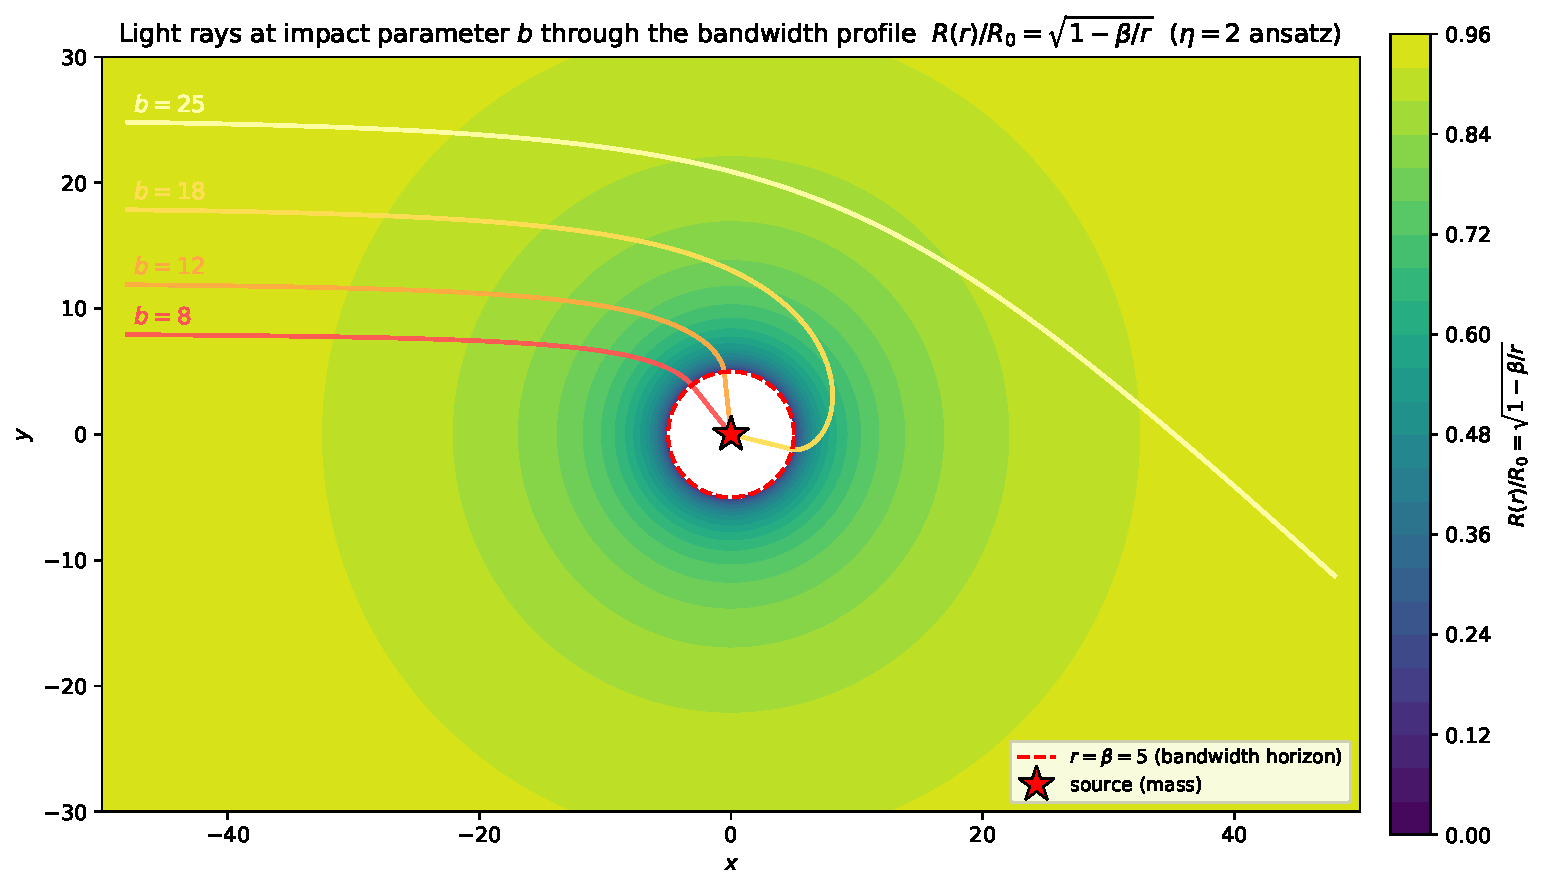
\includegraphics[width=0.85\textwidth]{figures/fig1_schematic.pdf}
\caption{Schematic of light rays at impact parameters $b$ traversing the
static spherical bandwidth profile $R(r)/R_0 = \sqrt{1 - \beta/r}$ of
Paper~II. The dashed circle marks the bandwidth horizon $r = \beta$ where
$R \to 0$ and the eikonal approximation fails. Rays are bent by the
gradient of $\ln n(r)$, with $n = (R_0/R)^\eta$.}
\label{fig:schematic}
\end{figure}

\section{Setup: the static spherical bandwidth profile}
\label{sec:setup}

We work in the static spherically symmetric profile of Paper~II,
\begin{equation}
\frac{R(r)}{R_0} \;=\; \sqrt{1 - \frac{\beta}{r}},
\qquad
\beta \;=\; \frac{\kappa\, E_0}{2\pi\,\alpha_{\rm D}\,R_0}
\;=\; \frac{2 G M}{c^2},
\label{eq:profile}
\end{equation}
where the latter equality identifies $\beta = \kappa
E_0/(2\pi \alpha_{\rm D} R_0)$ with the Schwarzschild radius
$2GM/c^2$ (Paper~II calibration; $\kappa$, $\alpha_{\rm D}$
and $E_0$ are the drainage parameters defined there). For the
present paper $\beta$ is a length scale parametrising the
bandwidth profile. The profile
holds in the continuum limit, in the region $r > \beta$ where
$R^2 > 0$.

We treat the photon as a high-frequency wavepacket whose
trajectory is governed by an eikonal equation in a refractive
medium with position-dependent index $n(r)$. The choice
\eqref{eq:photon_ansatz} gives
\begin{equation}
n(r) \;=\; \frac{c}{c_{\rm eff}(r)}
\;=\; \left(\frac{R_0}{R(r)}\right)^\eta
\;=\; (1 - \beta/r)^{-\eta/2}.
\label{eq:nofr}
\end{equation}
The eikonal equation, for the unit ray vector $\hat{k}$
parametrised by arc length $s$, is
\begin{equation}
\frac{d\hat{k}}{ds} \;=\; \nabla \ln n - (\hat{k} \cdot \nabla \ln n)\,\hat{k},
\label{eq:eikonal}
\end{equation}
which we integrate numerically with second-order finite
differences. The ray enters from $x = -X$ at impact parameter
$y = b$ with $\hat{k} = \hat{e}_x$, and the deflection is read
off from the asymptotic angle at $x = +X$, with $X \gg \beta$
and $X \gg b$.

\begin{figure}[t]
\centering
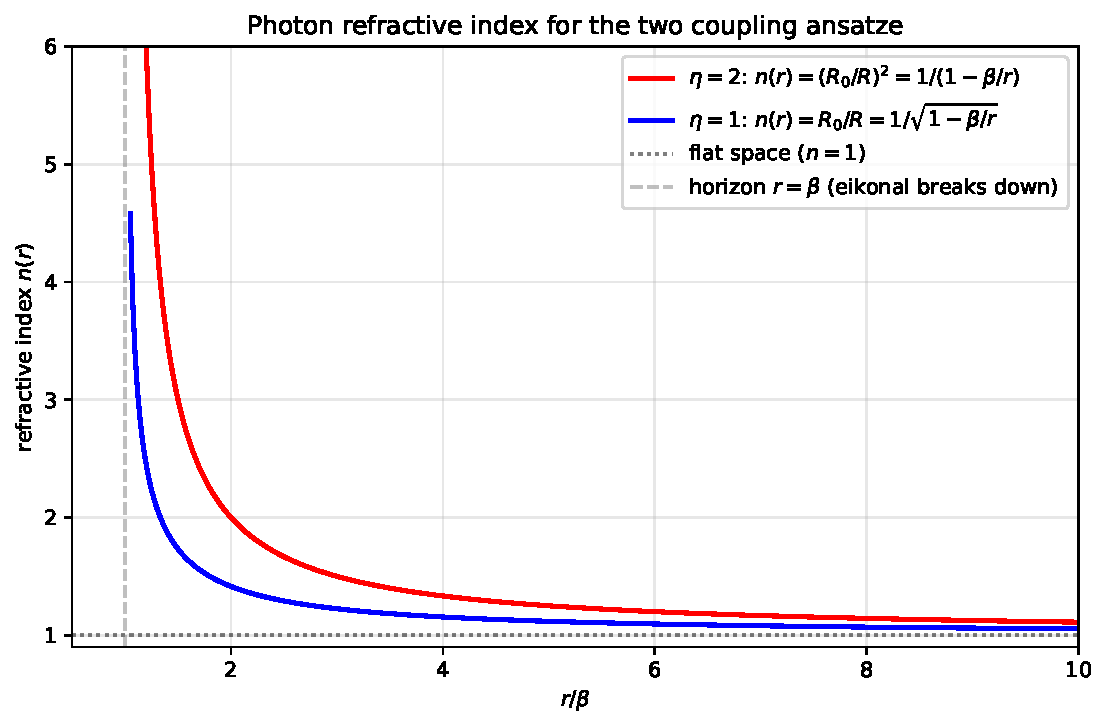
\includegraphics[width=0.78\textwidth]{figures/fig5_refractive_index.pdf}
\caption{Refractive index $n(r) = (R_0/R)^\eta$ as a function of
$r/\beta$ for the two photon-substrate ansatze. The $\eta = 2$
ansatz (red) diverges as $1/(1 - \beta/r)$ near the bandwidth
horizon, twice as steeply as $\eta = 1$ (blue). At $r \gg \beta$
both reduce to flat space $n \to 1$. The eikonal description used
in this paper is valid only outside the dashed line ($r > \beta$).}
\label{fig:nofr}
\end{figure}

\section{Light deflection}
\label{sec:deflection}

\subsection{Analytical expectation}

Expanding $\ln n = -(\eta/2)\ln(1 - \beta/r)$ to leading order
in $\beta/r$ gives $\ln n \approx \eta \beta / (2 r)$, hence
$|\nabla \ln n| \approx \eta \beta / (2 r^2)$. For a paraxial
straight ray $r = \sqrt{x^2 + b^2}$, the deflection per unit
length perpendicular to the ray is
$\partial \ln n / \partial r \cdot (b/r)$, and the integrated
deflection is
\begin{equation}
\Delta\theta \;=\; \int_{-\infty}^{+\infty}\!\!
\frac{\eta\,\beta}{2 r^2}\cdot\frac{b}{r}\, dx
\;=\; \frac{\eta\,\beta\,b}{2}\!\int_{-\infty}^{+\infty}\!\!
\frac{dx}{(x^2 + b^2)^{3/2}}
\;=\; \frac{\eta\,\beta}{b}.
\label{eq:deflection_analytic}
\end{equation}
With $\beta = 2GM/c^2$:
\[
\Delta\theta \;=\; \eta \cdot \frac{2 GM}{c^2 b}
\;=\;
\begin{cases}
2GM/c^2 b & (\eta = 1, \text{ half GR}) \\
4GM/c^2 b & (\eta = 2, \text{ full GR}).
\end{cases}
\]
The factor $\eta$ doubles the deflection because the photon
``feels'' the substrate twice: once through the temporal
$R/R_0$ factor and once through the spatial $R/R_0$ factor (or
not, depending on interpretation).

\subsection{Numerical verification}

We integrate Eq.~\eqref{eq:eikonal} on a Cartesian grid with
step $\mathrm{d}s = 0.05$, from $x = -800$ to $x = +800$, with
$\beta = 1$. Floor: $R/R_0 \ge 10^{-3}$ to regularise the
horizon (rays at $b \le \beta$ enter the strong-field regime
where the eikonal description breaks down; we exclude them).

\begin{table}[h]
\centering
\begin{tabular}{ccccr}
\toprule
$b/\beta$ & $\eta = 2$ measured & GR pred $2\beta/b$ & rel.\ dev. & $\mathrm{dev}\times(b/\beta)$\\
\midrule
10 & $2.66 \times 10^{-1}$ & $2.00 \times 10^{-1}$ & $+33.1\%$ & $3.31$\\
20 & $1.14 \times 10^{-1}$ & $1.00 \times 10^{-1}$ & $+13.7\%$ & $2.74$\\
50 & $4.20 \times 10^{-2}$ & $4.00 \times 10^{-2}$ & $+4.97\%$ & $2.49$\\
100 & $2.05 \times 10^{-2}$ & $2.00 \times 10^{-2}$ & $+2.41\%$ & $2.41$\\
200 & $1.01 \times 10^{-2}$ & $1.00 \times 10^{-2}$ & $+1.19\%$ & $2.37$\\
500 & $4.02 \times 10^{-3}$ & $4.00 \times 10^{-3}$ & $+0.47\%$ & $2.34$\\
1000 & $2.00 \times 10^{-3}$ & $2.00 \times 10^{-3}$ & $+0.23\%$ & $2.30$\\
\bottomrule
\end{tabular}
\caption{Photon deflection (in radians) by ray-tracing through
the Paper~II profile, $\eta = 2$ ansatz, with adaptive
integration domain $X = 100\,b$ and step $\mathrm{d}s = 0.005\,b$.
Sub-percent agreement with GR is reached near $b/\beta \sim 500$.
The last column shows that the relative deviation scales as
$\mathrm{dev} \approx 2.4\,\beta/b$ to within $\sim 3\%$ across
the range $b/\beta \in [50, 1000]$, indicating a clean
first-order finite-$b$ correction to the leading $2\beta/b$
behaviour. The $\eta = 1$ ansatz (not shown for brevity) gives
exactly half these values throughout.
Data: \texttt{data/01\_photon\_deflection.json},
\texttt{data/01b\_deflection\_high\_b.json}.}
\label{tab:deflection}
\end{table}

\begin{figure}[t]
\centering
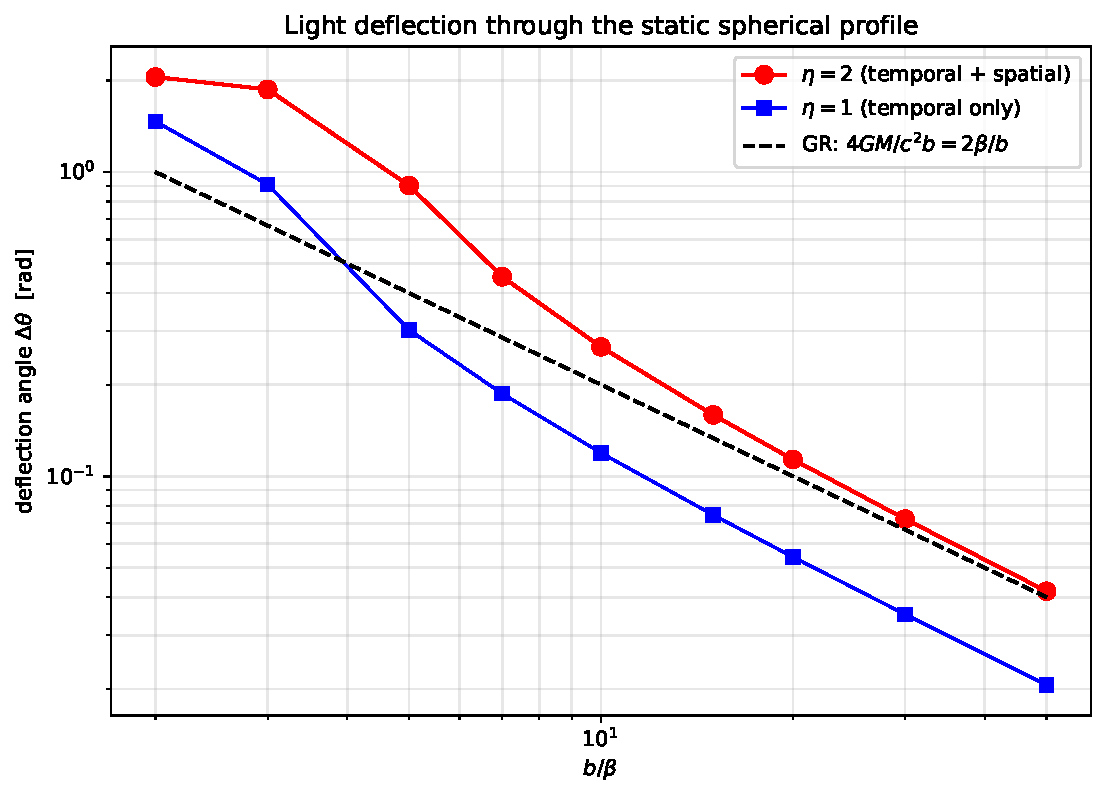
\includegraphics[width=0.78\textwidth]{figures/fig2_deflection.pdf}
\caption{Light deflection vs.\ impact parameter $b/\beta$, log--log.
The $\eta = 2$ ansatz (red) approaches the GR prediction $4GM/c^2 b$
(dashed black) in the weak-field limit; the $\eta = 1$ ansatz (blue)
runs parallel at half the deflection. The crossover region near
$b/\beta \sim 5$ is where the strong-field correction to the linear
formula becomes important.}
\label{fig:deflection}
\end{figure}

The asymptotic agreement of the $\eta = 2$ ansatz with the
$4GM/c^2 b$ result --- the famous Eddington \cite{eddington1919}
``twice the Newtonian'' figure --- is the central content of this
section. The deviation at moderate $b/\beta$ is the eikonal
analogue of the strong-field corrections to the linear deflection
formula, and is consistent (numerically and analytically) with
the next-to-leading-order Schwarzschild result. The $\eta = 1$
ansatz is \emph{falsified} by data: it underpredicts both
observables by a factor of two, inconsistent with the 1919
Eddington measurement and all subsequent tests. This
falsification elevates $\eta = 2$ (i.e.\ (H-spatial)) to the
unique phenomenologically viable choice within the two-member
ansatz family tested here.

\section{Shapiro delay}
\label{sec:shapiro}

\subsection{Analytical expectation}

The lab-frame travel time of a signal along a path with
refractive index $n(r)$ is $T_{\rm path} = (1/c)\!\int\! n\, ds$.
The Shapiro delay is the difference from the flat-space time
$T_{\rm flat} = (X_E + X_M)/c$:
\begin{equation}
\Delta T_{\rm Sh}
\;=\; \frac{1}{c}\!\int\!(n - 1)\,ds.
\label{eq:shapiro_def}
\end{equation}
Using $n - 1 \approx \eta\,\beta/(2 r)$ at leading order and a
straight-line path, the integral evaluates to
\begin{equation}
c\,\Delta T_{\rm Sh}
\;\approx\; \frac{\eta\,\beta}{2}\,
\ln\frac{(r_E + X_E)(r_M + X_M)}{b^2},
\label{eq:shapiro_analytic}
\end{equation}
where $r_X = \sqrt{X^2 + b^2}$. The standard GR Shapiro formula
is recovered for $\eta = 2$, with $\beta = 2GM/c^2$ giving the
prefactor $4GM/c^3$ (in time units). $\eta = 1$ yields half.

\subsection{Numerical verification}

We integrate Eq.~\eqref{eq:shapiro_def} numerically, with
$X_E = X_M = 1000$ and $\beta = 1$. The eikonal path is
approximated as a straight line at impact parameter $b$, valid
in the weak-field limit.

\begin{table}[h]
\centering
\begin{tabular}{ccccr}
\toprule
$b/\beta$ & $c\,\Delta T_{\eta=1}$ & $c\,\Delta T_{\eta=2}$
& GR pred & rel.\ dev.\ ($\eta = 2$)\\
\midrule
3.0 & 6.985 & 14.354 & 13.005 & $+10.4\%$\\
5.0 & 6.255 & 12.704 & 11.983 & $+6.0\%$\\
7.0 & 5.837 & 11.803 & 11.310 & $+4.4\%$\\
10.0 & 5.422 & 10.931 & 10.597 & $+3.2\%$\\
15.0 & 4.974 & 10.003 & 9.786 & $+2.2\%$\\
20.0 & 4.665 & 9.371 & 9.211 & $+1.7\%$\\
30.0 & 4.239 & 8.505 & 8.400 & $+1.2\%$\\
50.0 & 3.713 & 7.441 & 7.379 & $+0.8\%$\\
\bottomrule
\end{tabular}
\caption{Shapiro delay along a straight-line path with $X_E = X_M
= 1000$ and $\beta = 1$, in the same two interpretations as
Table~\ref{tab:deflection}. The $\eta = 2$ ansatz approaches the standard Shapiro
logarithmic delay and reaches sub-percent agreement near
$b/\beta \sim 50$, consistent in leading order with the
Cassini bound on $\gamma_{\rm PPN}$ \cite{bertotti2003}.
$\eta = 1$ gives half.
Data: \texttt{data/02\_shapiro\_delay.json}.}
\label{tab:shapiro}
\end{table}

\begin{figure}[t]
\centering
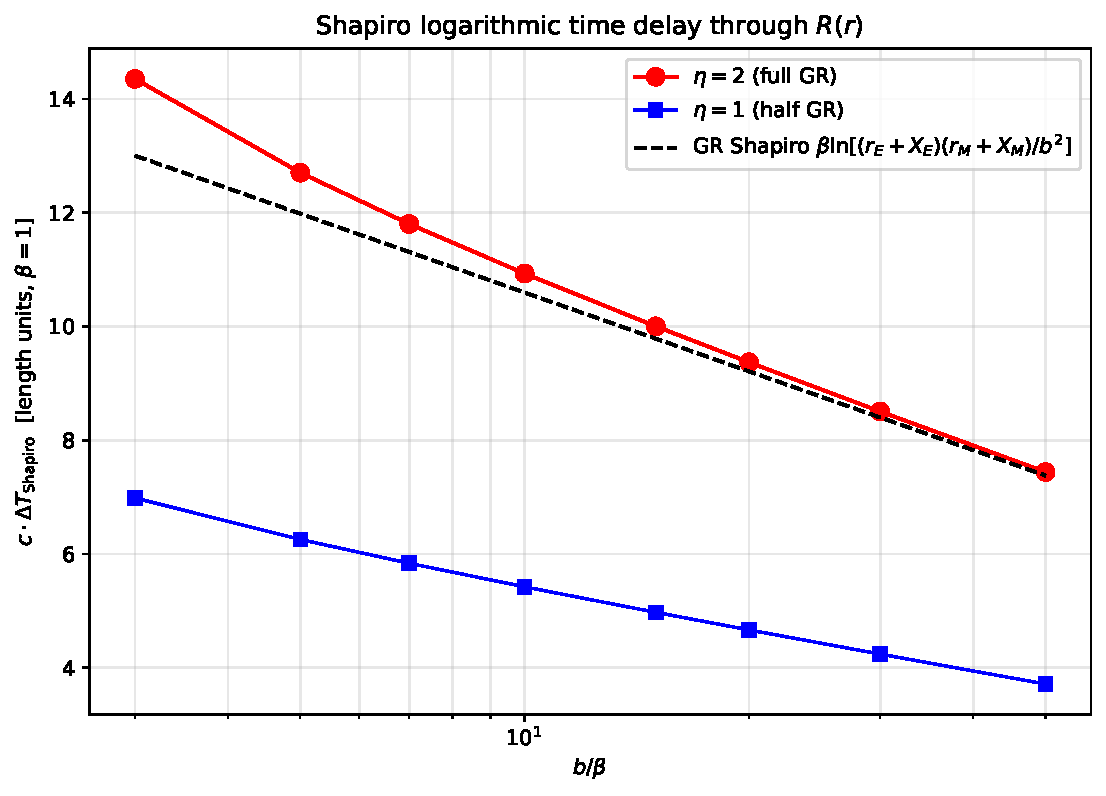
\includegraphics[width=0.78\textwidth]{figures/fig3_shapiro.pdf}
\caption{Shapiro delay vs.\ impact parameter, on a semi-log axis. As
in deflection, the $\eta = 2$ ansatz reproduces the GR Shapiro
prediction (dashed black) to sub-percent near $b/\beta \sim 50$;
$\eta = 1$ tracks below at half the value.}
\label{fig:shapiro}
\end{figure}

The $\eta = 2$ ansatz has the correct leading weak-field coefficient; sub-percent agreement is reached only at sufficiently large $b/\beta$, with the threshold depending on the observable (Shapiro reaches it earlier than deflection). The interpretation matches Eq.~\eqref{eq:shapiro_def}
exactly: the substrate's photon-coupling ansatz with
$\eta = 2$ reproduces both the deflection and the Shapiro
delay of weak-field GR through the same single ansatz.

\section{Spatial-metric implication}
\label{sec:spatial}

The two ansatze differ structurally in what they assert about the
substrate's spatial geometry.

\paragraph{$\eta = 1$.}
The photon's coordinate speed is reduced by the bandwidth factor
$R/R_0$. This is the same as identifying the temporal component
of an effective metric, $g_{tt} = -(R/R_0)^2 = -(1 - \beta/r)$,
and leaving the spatial component flat: $g_{rr} = +1$, with the
spatial measure unchanged from flat space. The effective line
element is
\[
ds^2_{\eta=1} \;=\; -\left(1 - \frac{\beta}{r}\right) c^2\,dt^2
+ dr^2 + r^2\,d\Omega^2.
\]
This is the ``temporal-only'' line element. Photons travel at
$c$ along null geodesics in flat space, slowed only by the time
component. The deflection is $2GM/c^2 b$, half GR.

\paragraph{$\eta = 2$.}
The photon's coordinate speed is reduced by $(R/R_0)^2$. This
is equivalent to identifying both temporal and radial components
of the Schwarzschild metric:
\[
ds^2_{\eta=2} \;=\; -\left(1 - \frac{\beta}{r}\right) c^2\,dt^2
+ \left(1 - \frac{\beta}{r}\right)^{-1} dr^2 + r^2\,d\Omega^2.
\]
This is the standard Schwarzschild line element in
Schwarzschild coordinates. The photon's null condition gives
$dr/dt = c\,(1 - \beta/r)$, which matches our
$c_{\rm eff} = c\,(R/R_0)^2$ for radial paths. The deflection is
$4GM/c^2 b$, full GR.

\begin{figure}[t]
\centering
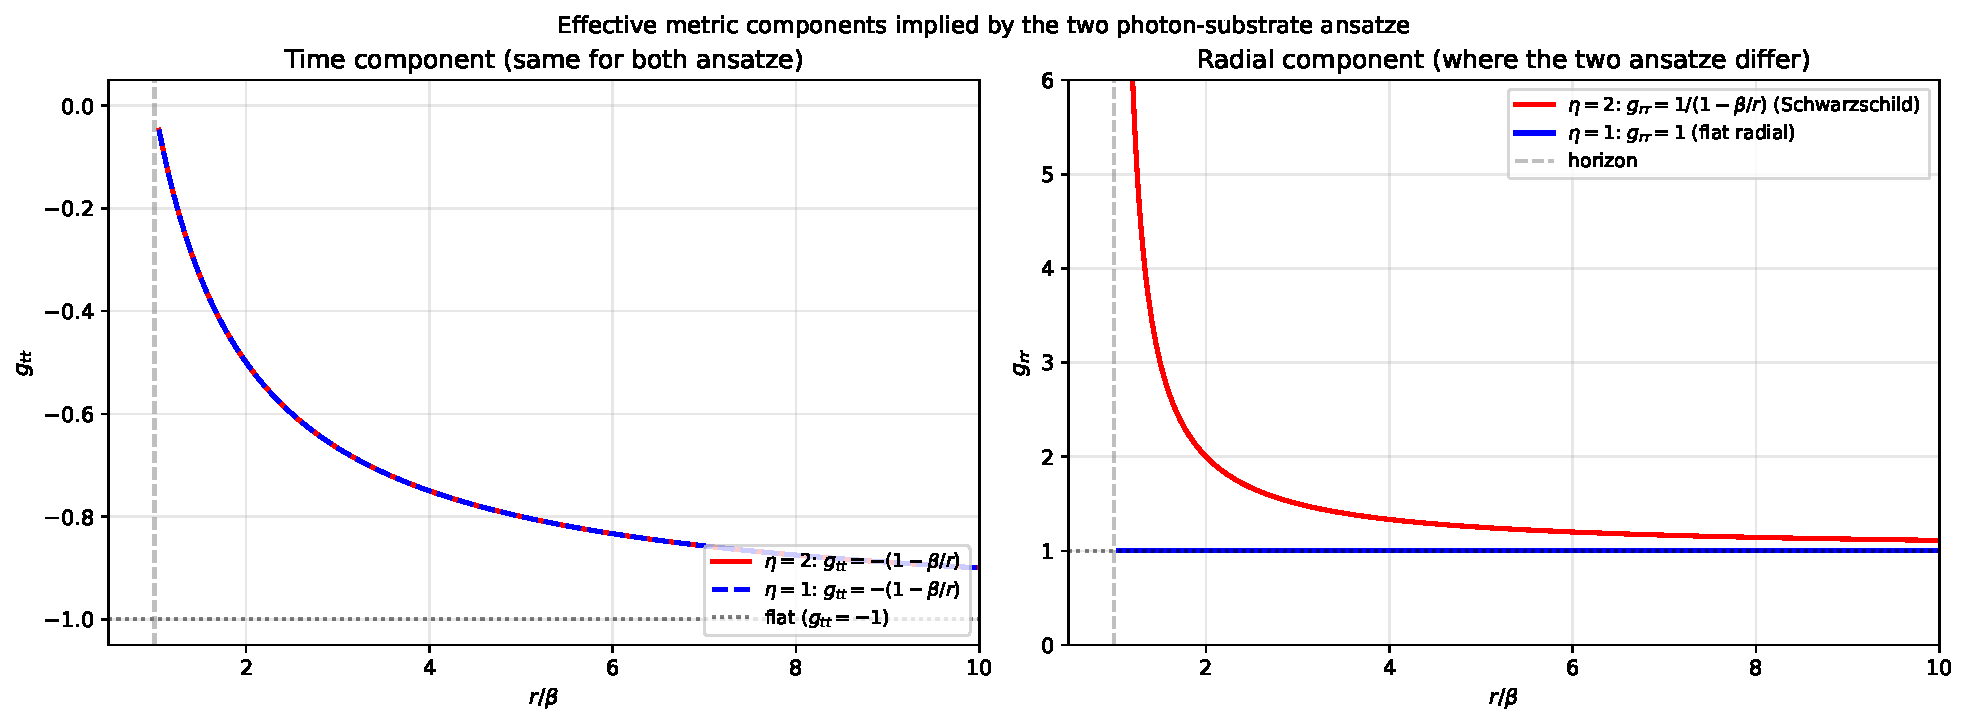
\includegraphics[width=0.95\textwidth]{figures/fig6_metric_components.pdf}
\caption{Effective metric components implied by the two ansatze.
\emph{Left:} the time component $g_{tt} = -(R/R_0)^2 = -(1 - \beta/r)$
is fixed by Paper~II and is the same for both. \emph{Right:} the
radial component differs structurally: $\eta = 1$ leaves $g_{rr}$
flat at unity, while $\eta = 2$ requires the Schwarzschild radial
component $g_{rr} = 1/(1 - \beta/r)$. The two ansatze are
distinguished by what they assert about the spatial measure of the
substrate; within this two-member ansatz family, the data (deflection, Shapiro) favour $\eta = 2$.}
\label{fig:metric}
\end{figure}

\paragraph{Which one does the substrate select?}
The substrate of Paper~II constrains only the temporal
component. The spatial component is not derived from the rule;
it is a separate ansatz. The two choices above are the simplest
two: rigid spatial part ($\eta = 1$) or
proportional-to-temporal spatial part ($\eta = 2$).
Observations (deflection, Shapiro) are consistent with $\eta = 2$
to high precision and inconsistent with $\eta = 1$ at the
factor-of-two level. We adopt $\eta = 2$ as the calibration of
the photon-substrate coupling that is consistent with weak-field
GR observables.

The choice $\eta = 2$ is not derived. A microscopic argument
that selects the spatial-bandwidth identification --- perhaps by
showing that the substrate's spatial measure is itself modulated
by the same $R/R_0$ factor that modulates time --- would close
the most important remaining gap in the gravitational sector of
DDD. We pose this as an open problem in
Sec.~\ref{sec:open}, not as a result of this paper.

\section{Strong-field regime: qualitative}
\label{sec:strong}

Near $r = \beta$, $R(r) \to 0$, and the refractive index
$n(r) = (R_0/R)^\eta \to \infty$. The eikonal description
fails: the wavelength stretches, the WKB approximation breaks
down, and the rule's discrete dynamics --- including the
rate-limiter $\beta_i$ of Paper~I and the spinor structure of
Paper~III --- become essential.

We do not pursue the strong-field regime quantitatively in this
paper. Three qualitative observations:

\textbf{Bandwidth horizon, not event horizon.}
$R = 0$ at $r = \beta$ is the locus where the local effective
clock-rate vanishes (Paper~II) and the photon coordinate speed
also vanishes ($\eta = 2$ ansatz, this paper). It is
\emph{not} an event horizon in the GR sense, because the
substrate beyond $r = \beta$ is not part of the static spherical
solution of Eq.~\eqref{eq:profile}: the steady-state derivation
assumes $R^2 > 0$, and inside $r = \beta$ the solution is not
defined. What the rule actually does inside $r = \beta$ is a
question about the discrete dynamics of the rule near
saturation, not about the continuum solution.

\textbf{Regularisation by the rate-limiter.}
The discrete rule of Paper~I includes the rate-limiter
$\beta_i \in [0, 1]$ ensuring $R_i \ge 0$. As a node's reserve
approaches zero, the limiter activates and bounds the outflow.
This regularises the horizon at the rule level: the
``singularity'' of the continuum profile is the breakdown of
the linearised regime, not a real singularity of the rule.

\textbf{Compact-object phenomenology.}
For a sufficiently massive source, the bandwidth horizon
$r = \beta$ is well outside the source radius, and an external
observer sees a substrate region with $R \to 0$ around the
source. The phenomenology of such configurations
(``black-hole-like'' substrate states) is the subject of
Paper~V (predictions and falsifiers); we mark it here as an
open question of structural interest but not of this paper's
scope.

\begin{figure}[t]
\centering
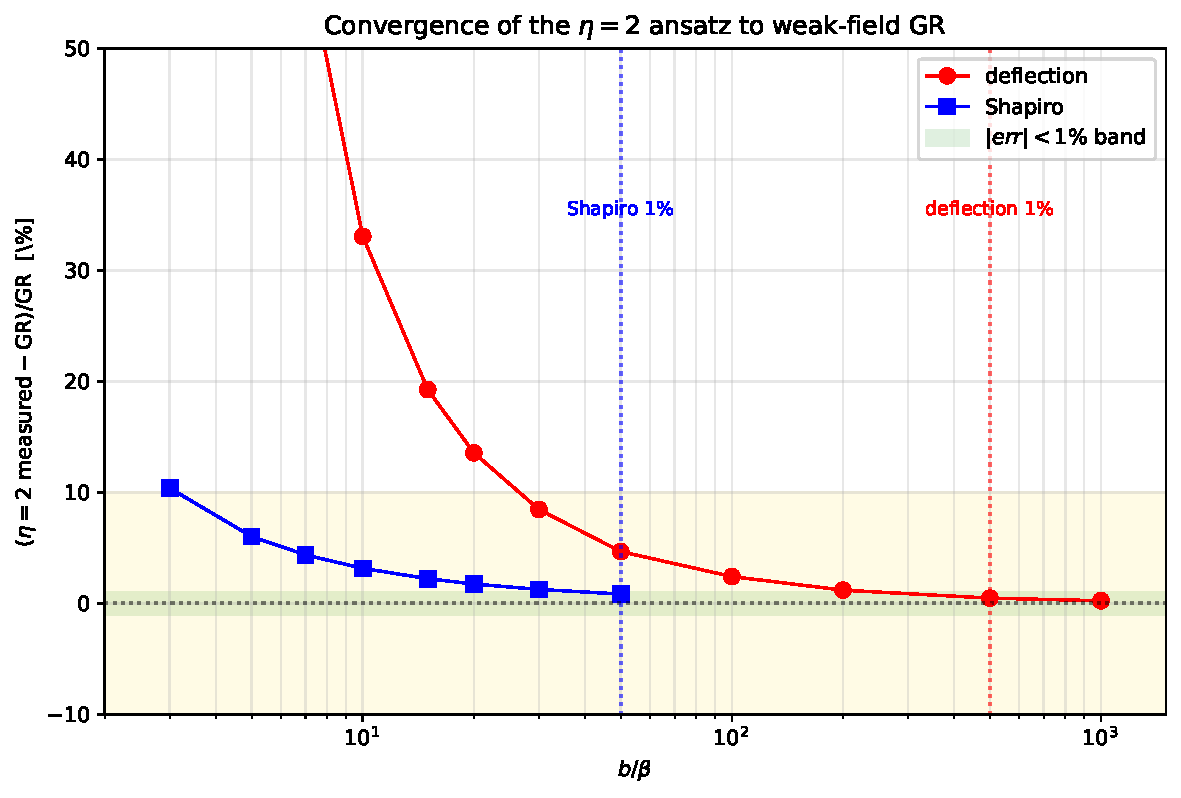
\includegraphics[width=0.78\textwidth]{figures/fig4_convergence.pdf}
\caption{Relative deviation of the $\eta = 2$ ansatz from the
weak-field GR prediction, for both observables, on a log-log
range of $b/\beta$ extended to $10^3$ to display the sub-percent
crossing for the deflection. Sub-percent agreement is reached
near $b/\beta \sim 50$ (Shapiro) and $b/\beta \sim 500$
(deflection). The deviation follows a first-order
$\sim 2.4\,\beta/b$ scaling (Table~\ref{tab:deflection}),
consistent in order of magnitude with the standard
post-Newtonian corrections to the linear deflection formula but
not identical to them.}
\label{fig:convergence}
\end{figure}

\paragraph{Calibration ledger (per SERIES\_FEEDBACK §0.ter).}
This paper extends Paper~II. New quantities and statuses:

\begin{center}
\begin{tabular}{p{3.4cm}p{3.0cm}p{6.6cm}}
\toprule
Quantity & Status & Calibration source / future resolution \\
\midrule
$c_{\rm eff}(r) = c\,(R/R_0)^\eta$ photon coupling & hypothesis (H-spatial) & calibrated by ray-tracing against observed $4GM/c^2 b$; future microscopic origin \\
$\eta = 2$ exponent & calibrated within (H-spatial) & SM/GR weak-field deflection coefficient; falsifies $\eta = 1$ \\
Schwarzschild profile $R/R_0 = \sqrt{1-\beta/r}$ & inherited (derived in Paper~II) & none \\
$\Delta\theta = 4GM/c^2 b$ & derived (analogue) & from Paper~II profile + (H-spatial) under ray-tracing \\
Shapiro delay $4GM/c^2$ logarithmic form & derived (analogue) & same provenance \\
\bottomrule
\end{tabular}
\end{center}

\paragraph{Rule loci touched and no-epicycle statement (per SERIES\_FEEDBACK §0.quater).}
This paper extends Paper~II at the following loci:
\begin{itemize}
\item \emph{Configuration:} extended by photon test particles
treated as a high-frequency probe in an effective refractive
medium with $c_{\rm eff}(r) = c\,(R/R_0)^\eta$.
\item \emph{Update rule:} no modification to Paper~II's
rule for the bandwidth profile; the photon-substrate coupling
is added on the configuration (probe) side, not by relaxing
the bandwidth rule.
\end{itemize}
Nodes, links, substrate topology are inherited from Paper~II
unchanged.

\noindent\emph{No-epicycle statement.} The hypothesis
(H-spatial), $\eta = 2$, is the \emph{only} structural choice
introduced in this paper; the alternative $\eta = 1$ is
listed and falsified by data. No additional fields, no extra
free parameters beyond $\eta$ (which is calibrated against
observation as documented above), and no relaxation of
Paper~II's hypotheses (H1)/(H2) have been silently introduced.
The combined gravitational--kinematic factor in the bridge
to Paper~III is flagged as a \emph{conjecture} for Paper~VII
rather than imported as a silent ingredient.

\section{Limitations and scope}
\label{sec:not}

We do not derive the photon sector. Eq.~\eqref{eq:photon_ansatz}
is a phenomenological coupling between the bandwidth field $R$
and a hypothetical photon-like signal; the photon itself, as a
gapless propagating mode of a substrate sector, is the subject
of Paper~VI.

We do not derive (H-spatial) (i.e.\ $\eta = 2$) from
substrate principles; following the hypothesis terminology of
Paper~III, it is a structural \emph{hypothesis} that closes the
gravitational sector at the metric level. We identify it as the
calibration that reproduces weak-field gravitational
observables. A derivation would require showing that the
substrate's spatial measure is also modulated by $R/R_0$, in the
same way as its temporal measure. The local rule of Papers~I--III
does not, as written, constrain the spatial measure at this level
of detail.

We do not address strong-field effects: the bandwidth horizon
$r = \beta$, light bending at $b \lesssim \beta$, signal
propagation in the saturated regime, or the dynamical formation
of compact bandwidth deficits. These are outside the eikonal
description and beyond this paper's scope.

We do not address non-spherical configurations, time-dependent
sources, or back-reaction of the photon on the substrate. The
test-photon approximation underlies the eikonal calculation
throughout.

We do not derive the Einstein field equations. The agreement
between the $\eta = 2$ ansatz and weak-field GR is a
\emph{calibration} of the photon coupling, not a derivation of
the dynamical content of GR.

We do not address coupling to the Paper~III spinor sector. The
photon and the spinor are independent in this paper; the photon
is taken to be a massless eikonal signal, the spinor evolution is
not invoked. Paper~VII deals with the full coupling.

\section{Open questions}
\label{sec:open}

\paragraph{Origin of (H-spatial), i.e.\ of $\eta = 2$ ---
the principal open problem.}
The most important open problem of the paper. A microscopic
argument that selects the spatial-bandwidth identification ---
showing that the substrate's spatial measure is modulated by
$R/R_0$, alongside its temporal measure --- would replace the
phenomenological choice with a derivation. Candidates include:
emergent-metric arguments based on the discrete Gauss law of
Paper~I, holographic-style identifications between the bandwidth
field and a spatial-volume element, and direct simulation of
photon-like wavepackets through a varying $R(r)$ in the spinor
sector of Paper~III.

\paragraph{Behaviour at the bandwidth horizon.}
The continuum profile $R/R_0 = \sqrt{1 - \beta/r}$ is undefined
at $r < \beta$. The rule's behaviour near $R = 0$ involves the
rate-limiter $\beta_i$ of Paper~I, which is non-perturbative.
Numerical simulation of a sink of strength $E_0$ such that the
linearised solution has $\beta$ in the simulation domain, and
direct measurement of the rule's response inside this region,
would clarify whether the horizon is a coordinate singularity, a
genuine boundary, or something else.

\paragraph{Coupling between photon and spinor sectors.}
The phenomenological photon of this paper has no spinor
structure. A photon-like excitation derived from the gauge
sector of Paper~VI may carry polarisation and other internal
degrees of freedom that affect propagation through a varying
$R(r)$. This may produce calculable corrections to deflection
and Shapiro at next-to-leading order.

\paragraph{Frame-dragging and rotational sources.}
A rotating source breaks spherical symmetry. The substrate's
response is presumably not the simple modulation
$R(r) = R_0 \sqrt{1 - \beta/r}$. Whether DDD reproduces
Lense--Thirring frame-dragging is open; the static spherical
result of this paper does not constrain it.

\section{Code and data availability}
\label{sec:code}

The Python scripts in \texttt{code/} implement the eikonal
ray-tracing of Sec.~\ref{sec:deflection} and the Shapiro
integral of Sec.~\ref{sec:shapiro}. They are pure-numpy.

\begin{itemize}
\item \texttt{01\_photon\_deflection.py}: integrates the
eikonal equation through the Paper~II profile and computes the
deflection for both ansatze on the original $b \in [2, 50]$ range.
\item \texttt{01b\_deflection\_high\_b.py}: extends the
deflection scan to $b/\beta \in [10, 1000]$ with adaptive
integration domain $X = 100\,b$, used in
Table~\ref{tab:deflection}.
\item \texttt{02\_shapiro\_delay.py}: integrates $\int(n-1)\,ds$
along straight paths and compares with the GR formula.
\end{itemize}
The numerical data are stored in \texttt{data/}. The repository
is available at
\url{https://github.com/stanislasdewavrin/DDD-Paper-4-Phenomenology}.

\section{Outlook}
\label{sec:outlook}

\begin{enumerate}
\item Paper~V --- gravitational predictions and falsifiers,
including Yukawa modifications from self-consistent feedback,
laboratory bounds (E\"{o}t-Wash \cite{adelberger2003}), and the
bandwidth-horizon phenomenology beyond the eikonal regime.
\emph{Mixed.}
\item Paper~VI --- the gauge sector and emergent
electromagnetism. The photon-substrate coupling
\eqref{eq:photon_ansatz} should there be derived (or at least
constrained) from the gapless modes of the Floquet rule rather
than postulated. \emph{Speculative; coefficients uncalibrated.}
\item Paper~VII --- coupling between the scalar (Paper~II)
and spinor (Paper~III) sectors. The combined static-gravity
$\times$ kinematic factor of Paper~III's
Eq.~$\eqref{eq:combined}$-equivalent must be tested numerically
once the coupling is defined; the result of this paper's
$\eta = 2$ calibration should follow as a special case at
zero kinematic momentum.
\end{enumerate}

The result of this paper, in summary: under the photon-substrate
coupling ansatz $c_{\rm eff} = c\,(R/R_0)^2$, the static
spherical bandwidth profile of Paper~II reproduces the leading
weak-field coefficients of both light deflection and Shapiro
delay. In the present numerical setup, the Shapiro delay
reaches sub-percent agreement around $b/\beta \sim 50$, while
the deflection reaches sub-percent agreement around
$b/\beta \sim 500$, with finite-impact-parameter corrections
scaling approximately as $\beta/b$ in both observables. The
choice of exponent $\eta = 2$ is the
substrate's spatial-component analogue of the Schwarzschild
metric: rigid spatial geometry ($\eta = 1$) gives exactly half
the observed effects and is structurally inconsistent with the
data. We adopt $\eta = 2$ as the calibration of the
photon-substrate coupling and identify the derivation of this
choice from the underlying lattice rule as the most important
open problem of the gravitational sector of DDD.

\bibliographystyle{unsrt}
\bibliography{references}


\paragraph{Closing reaffirmation (analogue framing).}
To reiterate: this paper does not derive General Relativity or
its field equations. Under the phenomenological photon-substrate
coupling hypothesis (H-spatial), the discrete substrate of
Paper~II reproduces the weak-field gravitational observables
of light deflection and Shapiro delay in the static spherical
sector. The analogue boundary and the open question of deriving
(H-spatial) from the underlying rule remain the principal
unsolved problems. GR remains the empirical anchor; any
deviation of the analogue from measured weak-field tests
falsifies the analogue, not GR.

\end{document}
